\renewcommand{\theequation}{\theenumi}
\begin{enumerate}[label=\arabic*.,ref=\thesubsection.\theenumi]
\numberwithin{equation}{enumi}
\item given that $\to$
\begin{align}
Z &= -3x + 4y
\\
\text{subjected to}
\\
x + 2y &\leq 8
\\
3x + 2y &\leq 12
\\
x  &\geq 0
\\
y &\geq 0
\end{align}
Comparing above equation to the gernelised form$\to$ 
\begin{align}
minZ &= c^t \vec{x}
\\
\text{subjected to}
\\
A\vec{x} &\preceq b
\\ 
\text{we can find $\to$ }
\\
c &= \myvec{-3\\ 4}
\\
A &= \myvec{1 & 2 \\ 3 & 2\\1 &0 \\ 0 & 1}
\\
b &= \myvec{8\\12\\ 0\\ 0}
\end{align}\\
Solution for the above equations can be find from the python code of Lenear programing 
\begin{lstlisting}
./optimization/codes
\end{lstlisting}
From the codes we get that the minimum value of the equation will be 12 at the point $\myvec{4 & 0}$.

\begin{figure}[!ht]
	\centering
	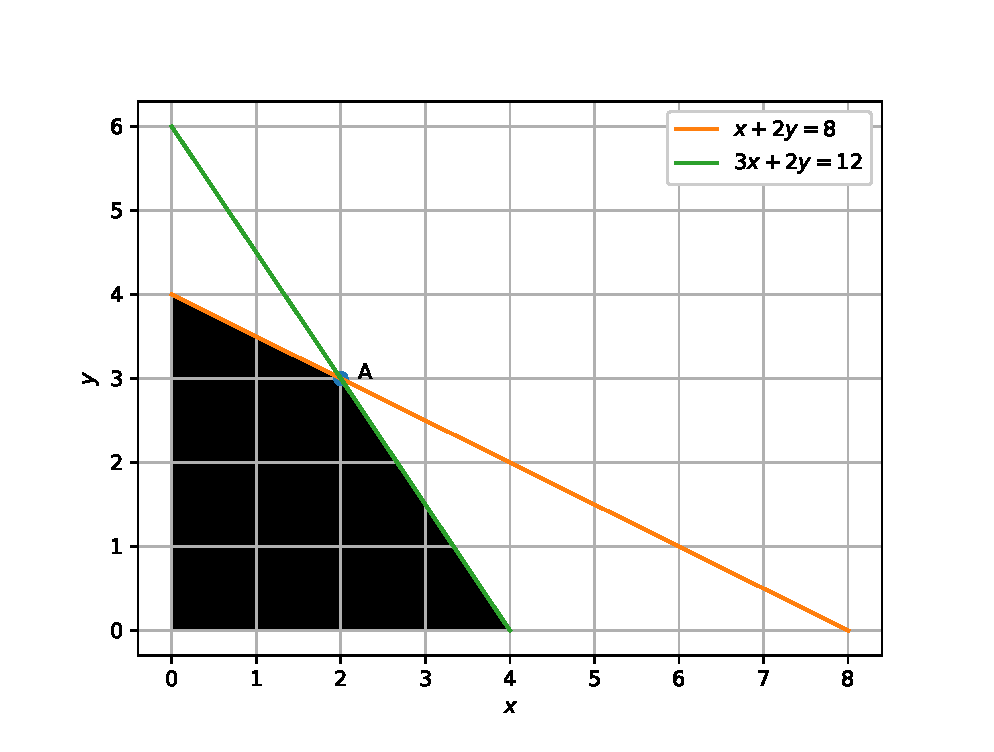
\includegraphics[width=\columnwidth]{./figures/lp4.eps}
	\caption{ lp4 }
	\label{fig:lp4}
	pythone codes for the above figure can be get from
	\begin{lstlisting}
	./optimization/figures/lp4.eps
	\end{lstlisting}	
\end{figure}
\end{enumerate}